\documentclass[]{scrreprt}%scrartcl
\usepackage{hyperref}
\usepackage{multirow}
\usepackage{listings}
\usepackage[pdftex]{graphicx}
\usepackage[tablegrid]{vhistory}
\usepackage{acronym}
\usepackage{titling}
\usepackage{booktabs}
\usepackage{amssymb}
\usepackage[disable]{todonotes} %draft
\usepackage{tablefootnote}


%%%%%%%%%%%%%%%%%%%%%%%%%%%%%%%%%%%%%%%%%%%%%%%%%%%%%%%%%%%%%%%%%%%%%%

%% DOCUMENT SETUP

%%%%%%%%%%%%%%%%%%%%%%%%%%%%%%%%%%%%%%%%%%%%%%%%%%%%%%%%%%%%%%%%%%%%%%

%document title
\newcommand{\docTitle}{ESP32 - Getting Started\\ToRaDes Smart Home implementation}

%document workpackage number
%e.g.: AP x.x
\newcommand{\docWPNumber}{AP 3}

%document status
%e.g.: Draft, Review or Final
\newcommand{\docStatus}{Draft}

%document dissemination level
%PU....Public, RE....Restricted
\newcommand{\docDissemination}{PU}

%document ID
%e.g. TR-AP-X_X-YY, X_X -> workpackage, YY -> number
\newcommand{\docID}{TR-AP-3$\_$*-01}

%changelog / history
\newcommand{\docChangelog}{


  \vhEntry{0.1}{27.01.17}{BA}{created}
  \vhEntry{0.2}{06.04.17}{BA}{ch. 6.1.1 Bluetooth Low Energy extended}
  \vhEntry{0.3}{10.04.17}{BA}{added RFC7668 chapter}
  \vhEntry{0.4}{17.04.17}{BA}{implementation approach RFC7668}
  \vhEntry{0.5}{03.05.17}{BA}{UDP6/MQTT-SN parts}
%  \vhEntry{0.7}{23.05.XX}{TJ}{draft}
%  \vhEntry{0.8}{23.05.XX}{TJ}{correction}
%  \vhEntry{0.9}{03.06.XX}{TJ}{Revised after review}
%  \vhEntry{1.0}{03.06.XX}{TJ}{Final version}

}


%%%%%%%%%%%%%%%%%%%%%%%%%%%%%%%%%%%%%%%%%%%%%%%%%%%%%%%%%%%%%%%%%%%%%%

%% GENERAL SETUP (NORMALLY NOT CHANGED)

%%%%%%%%%%%%%%%%%%%%%%%%%%%%%%%%%%%%%%%%%%%%%%%%%%%%%%%%%%%%%%%%%%%%%%

%%%% authors %%%%
\newcommand{\BA}{Benjamin Aigner}
\newcommand{\BAEmail}{aignerb}
\newcommand{\CV}{Chris Veigl}
\newcommand{\CVEmail}{veigl}
\newcommand{\TJ}{Thomas Jerabek}
\newcommand{\TJEmail}{thomas.jerabek}

%\usepackage{todonotes}
%
%\newcommand{\todoINFO}[1]{\todo[color=blue!25]{INFO: #1}}
%\newcommand{\todoIMPORTANT}[1]{\todo[color=red!25]{IMPORTANT: #1}}
%\newcommand{\todoREV}[1]{\todo[color=green!25]{REVIEWED: #1}}


\setlength\parindent{0pt}

\hypersetup{
	pdftitle  = {\docTitle},
	pdfkeywords = {\docTitle, Version \vhCurrentVersion from \vhCurrentDate},
	pdfauthor = {\vhAllAuthorsSet}
	}

%%%%%%%%%%%%%%%%%%%%%%%%%%%%%%%%%%%%%%%%%%%%%%%%%%%%%%%%%%%%%%%%%%%%%%

%% PREAMBLE PAGES

%%%%%%%%%%%%%%%%%%%%%%%%%%%%%%%%%%%%%%%%%%%%%%%%%%%%%%%%%%%%%%%%%%%%%%

\begin{document}
% 
% \title{ToRaDes - Technical Report \\ {\Huge \docTitle}}
% \includegraphics[height=20mm]{logo.png}
% \author{\vhListAllAuthorsLongWithAbbrev \\{University of Applied Sciences Technikum Wien}
% \\{H\"ochst\"adtplatz 6, A-1200 Vienna, Austria}
% \\{Email: {\texttt{\BAEmail, \TJEmail, \CVEmail}}}
% \\{\texttt{@technikum-wien.at}}}
% 
% \date{Version \vhCurrentVersion\ from \vhCurrentDate}
% \maketitle
% 
% \end{titlingpage}

\begin{titlepage}
	
	\includegraphics[height=20mm]{logo.png} \hfill
	\includegraphics[height=20mm]{fhtw.png}
	
	\centering
	\par\vspace{1cm}
	{\scshape\Huge ToRaDes \normalsize \par Toolbox for Rapid Development of Smart Homes and Assistive Technologies \par}
	\vspace{1cm}
	{\scshape\Large Technical Report\par}
	\vspace{1.5cm}
	{\huge\bfseries \docTitle \par}
	\vspace{2cm}
	{\Large
	\vhListAllAuthorsLongWithAbbrev \\{University of Applied Sciences Technikum Wien}
	\\{H\"ochst\"adtplatz 6, A-1200 Vienna, Austria}
	\\{Email: {\texttt{\BAEmail, \TJEmail, \CVEmail}}}
	\\{\texttt{@technikum-wien.at}}
	\par}
	\vfill
	{\large Version \vhCurrentVersion\ from \vhCurrentDate \par}
	\begin{flushright}
	 \includegraphics[height=30mm]{ma23.png}
	\end{flushright}
\end{titlepage}

%Version history on bottom of page

\chapter*{Document Information}

\begin{tabular}{|l|l|}
\hline
\textbf{Issue Date} & \textbf{\vhCurrentDate}\\ \hline
\textbf{Workpackage-Number} & \textbf{\docWPNumber}\\  \hline
\textbf{Status} & \textbf{\docStatus}\\  \hline
\textbf{Dissemination Level} & \textbf{\docDissemination} \\ \hline
\textbf{Document ID} & \textbf{\docID} \\ \hline
\end{tabular}

\section*{ToRaDes}
\textbf{Toolbox for Rapid Development of Smart Homes and Assistive Technologies} \\
This project has been funded by the Municipal Department 23 of the City of Vienna 
(Economic Affairs, Labour and Statistics - MA 23) in course of the 18th Call "Competence Teams for Research and Teaching".

\section*{Disclaimer}
The information in this document is provided as is and no guarantee or warranty is given that the information is fit for any particular purpose. The user thereof uses the information at its sole risk and liability. 

\vfill\nopagebreak
\parbox{\textwidth}{
\begin{versionhistory}
\docChangelog
\end{versionhistory}}
\clearpage

\tableofcontents
\clearpage


%%%%%%%%%%%%%%%%%%%%%%%%%%%%%%%%%%%%%%%%%%%%%%%%%%%%%%%%%%%%%%%%%%%%%%

%% DOCUMENT STARTS HERE

%%%%%%%%%%%%%%%%%%%%%%%%%%%%%%%%%%%%%%%%%%%%%%%%%%%%%%%%%%%%%%%%%%%%%%

\chapter{Pin Overview}
\begin{center}

\begin{figure}[htb]
  \centering
  \includegraphics[width=160mm]{img/esp32.png}
  \caption{ESP32S modules - pinout}
\end{figure}

\begin{figure}[htb]
  \centering
  \includegraphics[width=160mm]{img/esp32_sparkfun.png}
  \caption{Sparkfun ESP32 Thing - pinout}
\end{figure}

\end{center}

\chapter{Introduction}

\section{ESP-IDF Installation}

Due to the ongoing development of the ESP-IDF package, this procedure might change without further notice.
Therefore, the detailed procedure is not described here. Instead, the original documentation by Espressif is referenced.
Please use following links to set up the development environment:

\begin{description}
  \item[Linux] https://esp-idf.readthedocs.io/en/latest/linux-setup.html
  \item[Windows] https://esp-idf.readthedocs.io/en/latest/windows-setup.html 
  \item[MacOS X] https://esp-idf.readthedocs.io/en/latest/macos-setup.html
\end{description}

Due to the native support for the GNU toolchain (gcc,gdb,ld,...), a Linux system is recommended. A VM installation is
also possible, please refer to the VM's installation guides for using USB devices within the VM. Possible solutions:

\begin{itemize}
 \item Oracle VirtualBox (recommended)
 \item Parallels Desktop
 \item VMWare (Player, Enterprise,...)
\end{itemize}



\section{Setting up a project}
\label{sec:setting_up}

The best solution of starting with a new project is the idf-template \textit{https://github.com/espressif/esp-idf-template} \cite{ESP01}.
After unzipping or cloning, a few steps are necessary to start the template:

\begin{itemize}
 \item make menuconfig
 \item make all 
 \item make flash
 \item make monitor
\end{itemize}

\section{Debugging}

Since the ESP32 chip supports on-chip debugging via JTAG \footnote{Joint Test Action Group, used as synonym for IEEE 1149.1}, it is obvious to integrate the debugging facilities
within a common IDE. Espressif supports Eclipse integration (for compiling and flashing only), and describes the procedure in the ESP-IDF documentation. 
This chapter extends the documentation a little bit further to IDE debugging with Eclipse.

Assuming there is already an ESP32 project (see section \ref{sec:setting_up}), which can be built and uploaded, it is necessary to follow these steps to use Eclipse for compiling and uploading:

\begin{enumerate}
 \item Install Eclipse IDE for C/C++Developers (https://www.eclipse.org/downloads/eclipse-packages/ 
 \item Select $File\rightarrow Import$
 \item Select as import source: $C/C++ \rightarrow Existing\ Code\ as\ Makefile\ Project$ and press next.
 \item Type a project name and select $Existing Code Location$ to point to the project main folder.
 \item Select $Cross\ GCC$ as $Toolchain\ for\ Indexer\ Settings$
 \item Press $Finish$
\end{enumerate}

In addition, the default project settings have to be adjusted to fit the ESP32 toolchain.
Adjust the project properties via $Right-Click$ on the project, selecting "Properties":

\begin{enumerate}
 \item $C/C++\ Build \rightarrow Environment$: Press "Add" and define following variables:
    \begin{itemize}
      \item Name \textit{L}, Value \textit{1}
      \item Name \textit{IDF$\_$PATH}, Value \textit{Path to your IDF}; Note for Windows users: replace all backslashes with forward slashes
    \end{itemize}
 \item $C/C++\ Build \rightarrow Environment$: Adjust \textit{PATH}: add the path to the xtensa-esp32-elf/bin folder. 
 \item Top level of $C/C++\ Build$: Uncheck \textit{Use default build command} and use following build command: 
    \begin{lstlisting}[frame=single]
    bash ${IDF_PATH}/tools/windows/eclipse_make.sh
    \end{lstlisting}
    Note: Linux users don't need the prefix \textit{bash}
 \item $C/C++\ General \rightarrow Paths\ and\ Symbols \rightarrow Includes \rightarrow$: Press "Add" and use following path: 
    \begin{lstlisting}[frame=single]
      ${IDF_PATH}/components 
    \end{lstlisting}
 \item $C/C++\ General \rightarrow Preprocessor\ Include\ Paths \rightarrow Providers \rightarrow CDT\ Cross\ GCC\ Built-in\ Compiler\ Settings$:  
    Replace $\$\{COMMAND\}$ with $xtensa-esp32-elf-gcc$
 \item $C/C++\ General \rightarrow Preprocessor\ Include\ Paths \rightarrow Providers \rightarrow \\ CDT\ GCC\ Build\ Output\ Parser \rightarrow 
 Compiler\ command\ pattern$: Put following command to the text field:\\
    \begin{lstlisting}[frame=single]
      xtensa-esp32-elf-(gcc)|([gc]\+\+)|(clang)
    \end{lstlisting}
 \item "Apply" and close the Project Properties wsindow
 \item Right-Click on the project, $Make\ Targets \rightarrow Create$ and add a new target called \textit{flash} (it must be named exactly flash, otherwise it won't upload the program)
\end{enumerate}

After these steps, it should be possible to compile an example via $Project \rightarrow Build\ All$. The compilation process might need a few minutes the first time, because all the libraries
are built too. If the build is finished, upload the program to the ESP32 via right-Click on the project, $Make\ Targets \rightarrow Build...$ and selecting the previous defined \textit{flash} target.
To re-do the previous command, pressing the F9 button is also possible.

\textbf{Note: Please close all terminal windows while uploading, otherwise the upload will fail!}

Congratulations, the build environment is complete. It's time for debugging...
\\

The ESP32 provides all the necessary pins for JTAG debugging. The following table shows two different pin assignments, one for the bare ESP32 chip and one for
the Sparkfun ESP32 thing. In addition, the JTAG names and pin positions on the standardized 20pin header are shown: \hfill \\

\begin{tabular}{|l|l|l|l|}
\hline
\textbf{ESP32 pin name}	& \textbf{ESP32 Thing pin name} & \textbf{JTAG name} 	& \textbf{JTAG pin (20pol)} \\ \hline \hline

+3,3V			& +3,3V				& +3,3V / VTarget	& 1 \\ \hline
RESET			& CHIP$\_$PU			& SRST			& 3 \\ \hline
GND			& GND				& GND			& 4 \\ \hline
MTDI			& 12				& TDI			& 5 \\ \hline
MTMS			& 14				& TMS			& 7 \\ \hline
MTCK			& 13				& TCK			& 9 \\ \hline
MTDO			& 15				& TDO			& 13 \\ \hline
\end{tabular}
\hfill \\

It is necessary to use an OpenOCD compatible JTAG adaptor. This example is based on the JTAGKey Tiny from Amontec. Other adaptors might need different settings, please have a look at http://openocd.net/ .
Espressif provides a ported version of OpenOCD to support the ESP32 chip. Follow these steps to complete the OpenOCD installation:

\begin{enumerate}
 \item Download and compile the OpenOCD sourcecode with following commands:\\
  \begin{lstlisting}
    git clone --recursive https://github.com/espressif/openocd-esp32.git
    cd openocd-esp32
    ./bootstrap
    ./configure [options]
    make
    sudo make install [optional]
  \end{lstlisting}
  \item Copy the esp32.cfg file from $IDF\_HOME/doc/$ to the current OpenOCD folder
  \item Edit this file to use the available JTAG hardware by replacing\\
    $source [find\ interface/ftdi/tumpa.cfg]$ \\
    e.g. with \\
    $source [find\ interface/ftdi/jtagkey.cfg]$
  \item Start OpenOCD with following command (from the OpenOCD directory):\\
    \begin{lstlisting}
     ./src/openocd -s ./tcl -f ./esp32.cfg
    \end{lstlisting}
\end{enumerate}

After performing these steps, it is possible to use the commandline gdb with the ESP32. Sometimes, it might be annoying to
use the CLI \footnote{Command Line Interface}. So we will set up Eclipse to use the gdb for fancy debugging.

Please ensure, that the command \textit{xtensa-esp32-elf-gdb} is executable via the command line without the absolut path.
If not, change the \textit{PATH} environment variable, including the xtensa- toolchain.

Following steps are necessary to setup the debugger in Eclipse:

\begin{enumerate}
 \item Install the \textit{C/C+ GDB Hardware Debugging} plugin for Eclipse: \\
  $Help \rightarrow Install\ New\ Software...$
 \item Restart Eclipse and open the Debug Configurations dialog:\\
 $Run \rightarrow Debug\ configurations...$
 \item Add a new \textit{GDB Hardware Debugging} configuration
 \item Following changes are necessary:
  \begin{description}
   \item[Main] Click \textit{Search Project...} and select the .elf file of the project. Ensure that the \textit{Standard GDB Hardware Debugging Launcher}
   is used. It can be changed via \textit{Select other...} on the bottom of this dialog.
   \item[Debugger] Type in \textit{xtensa-esp32-elf-gdb} as \textit{GDB Command}. The command set is set to \textit{Standard}, the protocol version is \textit{mi}.
    Select the option \textit{Use remote target} and choose \textit{Generic TCP/IP} as JTAG Device. The hostname should be \textit{localhost} and the port number \textit{3333}.\\
    \textbf{Note: Core 0 is used via port 3333, Core 1 via port 3334}
   \item[Startup] Uncheck everything, except \textit{Load image} and \textit{Load symbols}. Both settings should be left to the default value (use project binary).
   \item[Source] Nothing to be changed here.
   \item[Common] Uncheck \textit{Launch in background} and check \textit{Debug} in \textit{Display in favorites menu}.
  \end{description}
\end{enumerate}

After performing these steps, debugging with Eclipse should be possible. Please ensure to follow these steps exactly in this order, otherwise it is possible to experience
troubles.

\textbf{Starting a debug session:}\\

\begin{enumerate}
 \item Connect the JTAG hardware to the ESP32
 \item Plug in the ESP32
 \item Plug in the JTAG hardware
 \item Start OpenOCD:
    \begin{lstlisting}
     ./src/openocd -s ./tcl -f ./esp32.cfg
    \end{lstlisting}
 \item Start the Eclipse debug session via the \textit{Debug} button
 \item Press at least one time \textit{Resume} and  \textit{Pause}, otherwise the debug state is inconsistent.
\end{enumerate}





%Ablauf:
%ESP anstecken
%JTAGKey anstecken
% openocd starten
% -> Eclipse starten & einmal resume/pause drücken


% \chapter{Examples}
% 
% 
% \chapter{Components}
% 
% \section{Bluetooth}
% 
% \section{WiFi}
% 
% \section{Flash}
% 
% \section{Security}
% 
% \subsection{Secure Boot}
% 
% \subsection{Encrypted Flash}
% 
% \subsection{Key Exchange / Device pairing}
% 
% \chapter{Cheatsheets}
% 
% \section{I/O access}
% 
% \section{Peripherals}
% 
% \section{FreeRTOS}

%\section{Bluetooth and WiFi}

\chapter{ToRaDes - Implementation details}

This chapter covers the necessary communication protocols, which can be used in combination with the ESP32 chip
and the ToRaDes system structure. The ESP32 provides a WiFi (802.11 b/g/n) and a Bluetooth (BLE/EDR 4.2) interface, which
will be utilized.
Concerning the low-power requirements and the provided interfaces, the communication between the modules will be covered by the
BLE hardware. The gateway functionality will be done via the WiFi hardware or an additional external Ethernet connection.

\section{Communication protocols}

The following figure shows a proposed structure of the layer model for the software developed in the context of the ToRaDes project.
The base for all communication is the BLE physical layer, the link layer and the L2CAP network layer. These parts are highlighted in blue and are provided
by Espressif via the ESP-IDF framework. There is nothing to be implemented by the project team.

On the left side, highlighted in green, the Bluetooth protocols which are standardized by the Bluetooth SIG are shown. These stack will not
be used in this implementation. There are currently no sufficient protocols, services or profiles which meet the criteria for this project.

On the right side of this figure, the proposed stack for this system is shown. Basically it is a 6LoWPAN network, based on a Bluetooth LowEnergy
hardware. On top of it, it is possible to implement IPv6 communication, which is standardized and will be more and more common for all network enabled
devices. As it is common, the IPv6 layer is used in conjunction with TCP or UPD. On top of this stack, there should be an implementation of
either MQTT or CoAP. Both protocols are designed for constrained and low power devices. Which protocol will be used is not defined by now.

At the top of the whole stack, the application is implemented. This application takes care of the other steps to provide a functional smart-home network
with all defined requirements.

\begin{figure}[htb]
  \centering
  \includegraphics[width=100mm]{img/stack_ipv6-ble.png}
  \caption{Proposed layers for Bluetooth Low Energy combined with IPv6}
\end{figure}

Following sections will give a detailed explanation of the functionality and implementation details/approaches for each layer of the proposed model.

\pagebreak
\subsection{Bluetooth Low Energy}

\textit{Bluetooth low energy (Bluetooth LE, BLE, marketed as Bluetooth Smart) is a wireless personal area network technology designed 
and marketed by the Bluetooth Special Interest Group aimed at novel applications in the healthcare, fitness, beacons, security, 
and home entertainment industries. Compared to Classic Bluetooth, Bluetooth Smart is intended to provide considerably reduced power 
consumption and cost while maintaining a similar communication range.} \cite{WP01}

Following figure shows the standardized system structure of a Bluetooth implementation. The ToRaDes software will only use the BLE part, as well as the L2CAP
function. Instead of using GAP, GATT or ATT, an IPv6 compatible layer will be implemented or adopted.

\begin{figure}[htb]
  \centering
  \includegraphics[width=100mm]{img/bt_core.png}
  \caption{Bluetooth Core Overview, \cite{BT01}}
\end{figure}

\subsubsection{BLE Profiles}

Bluetooth Low Energy data transmission is organized in so called \textit{Generic Attribute Profile} specifications.
GATT is organized in following hierarchy:
\begin{description}
 \item[Profile] The top entity of a BLE device's functionality is called profile. The profile contains at least one service.
 \item[Service] Services are standardized by the Bluetooth SIG. Each service provides a defined set of capabilities for the device.
 There are services providing IPv6 transport over BLE \cite{BT02} or localization services. A service may contain characteristics.
 \item[Characteristic] A characteristic is a detailed description of data payloads.
\end{description}

According to \cite{BT02}, the IPSP profile (which is used for the 6LoWPAN implementation over BLE) does not need services and characteristics.
Within the advertising data, only the IPSP profile is announced.


\subsubsection{IPv6 over BLE - RFC 7668} \label{sec:rfc7668}

\textit{
   Bluetooth Smart is the brand name for the Bluetooth low energy
   feature in the Bluetooth specification
   defined by the Bluetooth Special Interest Group.
   Bluetooth LE is a radio technology targeted for devices that operate
   with very low-capacity (e.g., coin cell) batteries or minimalistic
   power sources, which means that low power consumption is essential.
   Bluetooth LE is an especially attractive technology for Internet of
   Things applications, such as health monitors, environmental sensing,
   proximity applications, and many others.}

   \textit{
   Considering the potential for the exponential growth in the number of
   sensors and Internet connected devices, IPv6 is an ideal protocol for
   communication with such devices due to the large address space it
   provides.  In addition, IPv6 provides tools for stateless address
   autoconfiguration, which is particularly suitable for sensor network
   applications and nodes that have very limited processing power or
   lack a full-fledged operating system or a user interface.} 
\cite{RFC7668}


Compared to other Wireless Sensor Network (WSN) protocols, BLE chips, stacks and boards are widely available and cheaper.
Usually, the BLE stack does not provide a full network integration.
This disadvantage is covered by the RFC7668 specification, which allows a transparent integration of any BLE device within
an IPv6 network.
Considering the wide range of possibilities, following advantages arise with this implementation:

\begin{itemize}
  \item Transparent routing in existing networks
  \item Wide range of available tools, software and implementations
  \item Possibility of using different classes of communication protocols on top of IPv6 (UDP/TCP with MQTT, CoAP, HTTP,...)
  \item Low protocol overhead (only 2-12Bytes with the powerful IPv6 header compression \cite{RFC6282})
  \item Seamless integration with other IEEE802.15.4 protocols using IPv6
\end{itemize}


\textbf{Addressing}

BLE devices are usually addressed either by their MAC address or a random address (always 48bits).
IPv6 networks use a 128bit address, with a few constraints if local addresses are used:

Link-local addresses are used with a prefix (\textit{fe80::/10}), which reduces the available addressspace to 64bits (twice as much as IPv4).
In addition, a BLE-MAC address (48bits) is converted to 64bits with following procedure. As example, a BLE MAC with 00:11:22:33:44:55 is used:


    
\begin{center}
      \includegraphics[width=22.5mm]{img/ble1.png}
\end{center}
\begin{description}
 \item[Transform BLE MAC to EUI64] Add \textit{0xFF} and  \textit{0xFE} in the middle of the address:
    \begin{center}
      \includegraphics[width=30mm]{img/ble2.png}
    \end{center}
 \item[Add link-local address] Add the link-local prefix of \textit{fe80::/10} to the address:
    \begin{center}
      \includegraphics[width=30mm]{img/ble3.png}
    \end{center}
    The result is a link-local IPv6 address, which can be used to ping a device or connect to a specified service.
\end{description}

\textbf{Router/Gateway}


If a firmware provides the IPSP profile and implements the RFC7668 specification, a gateway to other IPv6 networks is necessary.
It might be possible to implement such a gateway within the ESP32 (it has BLE and WiFi), currently this is not possible.
Currently a different approach is used:

The Linux kernel provides already the necessary infrastructure to establish a connection to BLE devices with IPv6.
This is done by loading a kernel module and establishing a connection to one or more BLE devices \cite{NORDIC2}:

\begin{lstlisting}[frame=single,language=bash,basicstyle=\footnotesize] 
modprobe bluetooth_6lowpan
echo 1 > /sys/kernel/debug/bluetooth/6lowpan_enable
hciconfig hci1 reset
echo "connect 24:0A:C4:04:B0:D2 1" > /sys/kernel/debug/bluetooth/6lowpan_control
echo "connect 24:0A:C4:04:B1:AA 1" > /sys/kernel/debug/bluetooth/6lowpan_control
echo "connect 24:0A:C4:04:B1:32 1" > /sys/kernel/debug/bluetooth/6lowpan_control

ping6 -I bt0 fe80::240a:c4ff:fe04:b132
ping6 -I bt0 fe80::240a:c4ff:fe04:b1aa
ping6 -I bt0 fe80::240a:c4ff:fe04:b0d2
\end{lstlisting}

After a successful connect, the linux kernel creates a new network device (\textit{bt0}), which is used to communicate with the BLE devices.


\subsubsection{Implementation Approach}

The esp-idf provides a fully functional network stack, implemented via lwIP \cite{LWIP01}. This network stack provides following protocols, which are used either
by the esp-idf and/or the ToRaDes RFC7668 implementation:

\begin{itemize}
  \item IPv4 and IPv6
  \item UDP and UDP6
  \item 6LoWPAN
  \item ICMP/IGMP
  \item DNS
  \item Network interface management
\end{itemize}

\begin{figure}[htb]
  \centering
  \label{img:ble_to_lwip}
  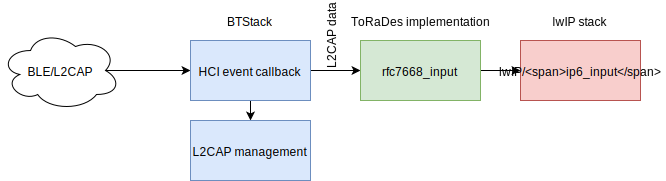
\includegraphics[width=100mm]{img/ble_to_lwip}
  \caption{BLE integration with lwIP}
\end{figure}

Figure \ref{img:ble_to_lwip} depicts the integration of BLE, the L2CAP handler within BTStack and the implementation of lwIP.
Reducing the modifications of the lwIP stack to a minimum, a new network interface was implemented. Therefore, no existing code of lwIP was modified, not even the build files.
It is planned to merge these additions to the upstream branch of lwIP. The new netif (\textit{rfc7668.c}) includes following functionalities, based on the 6lowpan network interface:
\begin{itemize}
 \item Address conversation (see chapter \ref{sec:rfc7668}, \textit{Addressing}) - RFC4862
 \item IP header compression/decompression - IPHC (based on 6lowpan implementation, RFC6282 \cite{RFC6282})
 \item Management methods (interface init,...)
\end{itemize}

Using this new netif is easy, a user/developer needs following two API methods for communicating with lwIP's stack and upper layers:

\begin{lstlisting}[frame=single,language=C,basicstyle=\footnotesize] 
//define a callback function, which handles output data
netif->linkoutput(netif, p_frag)
//input function, which is used to process incoming data
err_t rfc7668_input(struct pbuf * p, 
  struct netif *netif, const ip6_addr_t *src)
\end{lstlisting}

These two methods are used to glue the Bluetooth stack with the lwIP stack.
Currently two different Bluetooth stacks maybe used with the ESP32 controller:
\begin{description}
 \item[Bluedroid] Bluedroid is currently widely used by the Android OS. It provides a wide range of implemented services, profiles and APIs.
 Unfortunately, it is hard and time consuming to implement a new L2CAP service within the stack. Implementing the RFC7668 communication would require deep
 modifications of the Bluedroid code, which might lead to incompatibilities to the ongoing development within the ESP-IDF. Due to these disadvantages, this implementation
 uses the second option. In future updates, a switch back to the free and open-source stack might be possible.
 \item[BTStack] This stack is developed by the Swiss company Bluekitchen. It is available as open-source software, but it is limited to personal or academic use. A commercial
 usage requires a license (about 1CHF fee each device in small-amounts). BTStack uses a direct communication to the Bluetooth controller via the HCI-H4\footnote{\textbf{H} ost \textbf{C}ontroller \textbf{I}nterface} interface. Adding a new L2CAP service is easily done with the well-documented API.
\end{description}


The basic principle of adding and activating the RFC7668 interface is depicted in the following listing:

\begin{lstlisting}[frame=single,language=C,basicstyle=\footnotesize] 
//setup l2cap for IPSP support
//BT_PSM_IPSP => 0x0023 /* Internet Protocol Support Profile  */
//WARNING: change security level 0!!! Currently used for testing
//l2cap_ipsp_cb -> callback for this L2CAP service
//used to establish a connection and sending received data to rfc7668_input
l2cap_le_register_service(l2cap_ipsp_cb,PSM_IPSP,LEVEL_0);

//turn BLE interface on
hci_power_control(HCI_POWER_ON);

//actvate lwIP stack
//not used, but possible: callback if init is finished
tcpip_init(NULL, NULL); 

//add the lwIP network interface
netif_add(&rfc7668_netif, 
    /* fields are only available if compiled with IPv4
    we DO NOT support IPv4 -> NULL */
    #if LWIP_IPV4
      NULL,NULL,NULL,
    #endif /* LWIP_IPV4 */
    /* provide interface init and input function */
    NULL, rfc7668_if_init, rfc7668_input);

//add an IPv6 address (based on the BLE-MAC)
netif_add_ip6_address(&rfc7668_netif,&ip6addr_local,NULL);
//add an interface name
rfc7668_netif.name[0] = 'B';
rfc7668_netif.name[1] = 'T';

//link the network interface to the sending function
rfc7668_netif.linkoutput = rfc7668_send_L2CAP;
\end{lstlisting}

This procedure is necessary to bring up this interface.
A different Bluetooth stack (e.g. Bluedroid) might need a different activation of the corresponding L2CAP activation and callback handling.
The linkage between BTStack and lwIP needs one additional part (despite a normal L2CAP connection activation), the processing of gathering L2CAP data
and transfer it to lwIP. Following listing depicts the callback \textit{$l2cap\_ipsp\_cb$}, if the incoming packet is a HCI event of the type \textit{$L2CAP\_DATA\_PACKET$}:

\begin{lstlisting}[frame=single,language=C,basicstyle=\footnotesize] 
//L2CAP data packet on an established channel
case L2CAP_DATA_PACKET:	
	//determine if the address type is public
	//(different address modification in the linux kernel)
	if(ipsp_addr_type == BD_ADDR_TYPE_LE_PUBLIC)
	{
		ble_addr_to_eui64((uint8_t *)src.addr, peer_addr, 1);
	} else {
		ble_addr_to_eui64((uint8_t *)src.addr, peer_addr, 0);
	}
	
	//allocate a lwIP pbuf
	p = pbuf_alloc(PBUF_RAW, 127, PBUF_RAM);
	//payload: incoming packet
	p->payload = packet;
	//length: size of the incoming packet
	p->len = size;
	#if LOWPAN_BLE_DEBUG_L2CAP_CB
		printf("L2CAP: len: %d, tot_len: %d\n",p->len,p->tot_len);
	#endif
	//feed this packet to the network interface
	rfc7668_input(p,&rfc7668_netif,&src);
\end{lstlisting}

%inkscape --without-gui --export-pdf=dfs-task-structure-eval.pdf dfs-task-structure-eval.svg

With these modifications, it is already possible to process ICMPv6 pings with the ESP32. Other, upper layer, protocols will work too, if they use IPv6.
Due to power contraints and minimum data transfer, the ToRaDes implementation is based on UDPv6. Adding all protocol overhead from MQTT to lower layers (including IPv6 dest and src addresses),
a typical dataframe consists of 65 Bytes (payload "ON").
There might be an additional overhead, added by the DTLS integration.

\subsection{MQTT/MQTT-SN}

MQTT \footnote{\textbf{M}essage \textbf{Q}ueue \textbf{T}elemetry \textbf{T}ransport} is an ISO standardized protocol (ISO/IEC PRF 20922, \cite{MQ01}), which is based on the publisher/subscriber model.
A central management unit, called \textit{Broker}, is used to distribute messages to subscribed clients. MQTT uses a TCP/IP connection and support following methods for data handling and management:

\begin{description}
 \item[Connect] Connect to a MQTT broker
 \item[Disconnect] Disconnect from a MQTT broker
 \item[Subscribe] Subscribe to a specific topic. Wildcards maybe used.
 \item[Unsubscribe] Unsubscribe from a specific topic.
 \item[Publish] Publish data to a topic.
\end{description}

\subsubsection{Topics}

Publish and subscribe uses so called \textit{topics}, which are data points to clarify a destination of published data.
Topic description are textual names, seperated by slashes (/).

According to \cite{GH01}, wildcards might be used to subscribe to more than one topic:

\begin{description}
 \item[$A/\#$] Subscribe to topic A and every topic beneath A
 \item[$A/+$] Subscribe to topics direct beneath A, but not A itself
 \item[$A/+/\#$] Subscribe to all topics beneath A, but not A itself
\end{description}

Within the ToRaDes implementation, MQTT has a major disadvantage: it uses TCP/IP. With TCP/IP a threeway-handshake is necessary,
which increases the wake-up time for contrained nodes.

\subsubsection{MQTT-SN}

Fortunately, MQTT provides an additional specification for sensor networks, called MQTT-SN \cite{MQ02}.

\textit{"MQTT-SN is designed to be as close as possible to MQTT, but is adapted to the peculiarities of a wireless com-
munication environment such as low bandwidth, high link failures, short message length, etc. It is also optimized
for the implementation on low-cost, battery-operated devices with limited processing and storage resources."}\cite{MQ02}

Due to the limits of sensor networks, especially the possibility of sleeping clients, MQTT-SN extends the client states to a structure, which is depicted
in Figure \ref{img:mqtt-sn-state}.

\begin{figure}[htb]
  \centering
  \label{img:mqtt-sn-state}
  \includegraphics[width=100mm]{img/mqtt-sn-state}
  \caption{MQTT-SN state diagram, source \cite{MQ02}}
\end{figure}

Due to the protocol differences between MQTT and MQTT-SN, a gateway software is necessary.
In the project context of ToRaDes, the Paho software is used.

\subsection{Paho - MQTT-SN gateway}

Paho (originated within the Eclipse software project) provides a gateway for interfacing MQTT-SN to a MQTT broker.
Currently, Paho does NOT provide the possibility of using UDP6 sockets for the sensor network.

Within the ToRaDes project, the paho gateway was modified to support UDP6 as well as UDP4.
The implementation is basically a modification of address handling and socket operations.

The modifications will be more tested and merged to the upstream branch.

\subsection{TLS/DTLS}

The TLS/DTLS implementation is currently not completed. The documentation will be added as soon as the implementation is finished.

%TODO: TLS/DTLS -> MQTT mit TLS, MQTT-SN mit DTLS

\subsubsection{Implementation Approach}

The full ToRaDes smart home implementation is currently not completed. The documentation will be added as soon as the implementation is finished.

%TODO: host seite / ESP32 seite
%TODO: layering mit ,mbedtls/lwip/dtls/...


\section{Pairing}

%TODO: wie machen wir hier den schlüsselaustausch bzw das BT pairing?

\section{Over the air updates (OTA)}

%TODO: wie wird OTA gemacht? Z.B. Wifi?!?

\section{Key management}

%TODO: DTLS?!?

\section{Module differentiation}

%TODO: müsste eigentlich über ein MQTT topic gehen oder?


\chapter{Smart Home Modules}

This chapter specifies all current available or developing smart home modules, developed within the ToRaDes project.
Each module pages contain specifications, module pictures, typical applications and schematic/PCB documentation.
ToRaDes Smart Home (TSH) module names follow this naming convention:

\subsubsection{Naming convention}
\begin{center}
\textbf{TSH-xx-yyyy-zz} 
\end{center}
\begin{description}
 \item[xx] Mounting option. Currently available:
    \begin{description}
      \item[HS] Top-hat rail mounting (TS35)\footnote{German: Hutschiene}.
      \item[UP] In-wall module\footnote{German: Unterputz}.
      \item[AP] Wall-mounted module\footnote{German: Aufputz}
    \end{description}
 \item[yyyy] Module type, no further specification.
 \item[zz] Revision, starting with \textit{01}.
\end{description}

\section{Actuators}

%%%%%%%%%%%%%%%%%%%%% NEW MODULE %%%%%%%%%%%%%%%%%%%%%%%%%%%
\newpage
\subsection{8x Relay Module - TSH-HS-R801-01}

\begin{figure}[htb]
  \centering
  \label{img:TSH-HS-R801-01}
  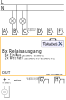
\includegraphics[width=50mm]{img/mod/TSH-HS-R801-01.png}
  \caption{TSH-HS-R801-01}
\end{figure}

The TSH-HS-R801-01 module is a top-hat rail (TS35) module, which provides 8 independent output. Six outputs provide a SPST-NO (single contact, normally opened) configuration,
two outputs provide a SPDT configuration (single pole, double throw). The module is compatible with all TSH modules and uses an external power supply of 5-15VDC (max 1.5W).

\newpage
\subsubsection{Specifications}

The TSH-HS-R801-01 relay module provides following specifications:

\begin{table}[h!]
\centering
\label{TSH-HS-R801-01-specs}
\begin{tabular}{|l|l|l|}
 \hline
Characteristics                                                                                  & Item                       & Specifications                                                                                                                                                                              \\ \hline \hline
\multirow{3}{*}{Dimensions}                                                                      & Width                      & 72mm (4TE)                                                                                                                                                                                  \\ \hline
                                                                                                 & Length                     & 90mm                                                                                                                                                                                        \\ \hline
                                                                                                 & Height                     & 63mm                                                                                                                                                                                        \\ \hline
\multirow{3}{*}{\begin{tabular}[c]{@{}l@{}}Electrical\\ Input\end{tabular}}                      & Power                      & \begin{tabular}[c]{@{}l@{}}1.5W (with both SPDT contacts)\\ 0.5W (only SPST contacts)\end{tabular}                                                                                          \\ \hline
                                                                                                 & Voltage                    & 5-15VDC                                                                                                                                                                                     \\ \hline
                                                                                                 & Current                    & \begin{tabular}[c]{@{}l@{}}300mA (@5V, with both SPDT contacts)\\ 125mA (@12V, with both SPDT contacts)\\ \\ 100mA (@5V, SPST contacts only)\\ 40mA (@12V, SPST contacts only)\end{tabular} \\ \hline
\multirow{4}{*}{\begin{tabular}[c]{@{}l@{}}Electrical Rating\\ SPST contacts (A-F)\end{tabular}} & Nominal switching capacity & 8A / 250VAC (resistive load)                                                                                                                                                                \\ \hline
                                                                                                 & Maximum switching power    & 2000VA (resistive load)                                                                                                                                                                     \\ \hline
                                                                                                 & Rating AC                  & 8A / 250VAC (resistive load)                                                                                                                                                                \\ \hline
                                                                                                 & Rating DC                  & 5A / 30VDC                                                                                                                                                                                  \\ \hline
\multirow{4}{*}{\begin{tabular}[c]{@{}l@{}}Electrical Rating\\ SPDT contacts (G-H)\end{tabular}} & Nominal switching capacity & 16A / 240VAC (resistive load)                                                                                                                                                               \\ \hline
                                                                                                 & Maximum switching power    & 3700VA (resistive load)                                                                                                                                                                     \\ \hline
                                                                                                 & Rating NO contact          & 16A / 240VAC                                                                                                                                                                                \\ \hline
                                                                                                 & Rating NC contact          & 8A / 240VAC                                                                                                                                                                                 \\ \hline
\end{tabular}
\end{table}

\subsubsection{MQTT - API}

TBD...
\newpage

\subsubsection{Applications}

The relay module maybe used for different loads. The maximum output rating is listed in the specifications.
Following use cases might be possible:

\begin{itemize}
 \item Lamp switching
 \item Blindings
 \item HVAC applications
 \item ...
\end{itemize}

\begin{center}
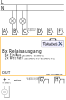
\includegraphics[width=50mm]{img/mod/TSH-HS-R801-01.pdf} 
\end{center}




\subsubsection{Schematic}
  
\includegraphics[width=0.96\textwidth]{img/mod/TSH-HS-R801-01-sch.pdf}

\begin{table}[h!]
\centering
\label{TSH-HS-R801-01-pins}
\begin{tabular}{|l|l|l|}
\hline
WROOM pin	& Module pin 	& Description \\ \hline \hline
EN / 3		& SW 1		& Reset button (within case), header P1, pin 5 \\ \hline
IO0 / 25	& SW 2		& Button 1, unload/pair \\ \hline
IO32 / 8	& SER		& SR$_{[1]}$, serial data \\ \hline
IO33 / 9 	& RCLK		& SR, clock input storage register \\ \hline
IO25 / 10	& G		& SR, output enable \\ \hline
IO26 / 11	& SRCLK		& SR, clock input \\ \hline
IO27 / 12	& SRCLR		& SR, reset (active LOW) \\ \hline 
IO14 / 13	& 7G		& Relay G \\ \hline 
IO12 / 14 	& 8G		& Relay H \\ \hline 
IO4 / 26	& DIO4		& IO4, header P1, pin 6 \\ \hline
RXD0 / 34	& RXD		& UART RX, header P1, pin 3 \\ \hline 
TXD0 / 35	& TXD		& UART TX, header P1, pin 4 \\ \hline
\end{tabular}
\\
\footnotesize [1] - Shift Register, 74HC595
\caption{TSH-HS-R801-01 ESP32 pin assignment}
\end{table}
 
\hfill \\

The relay outputs A to F are bi-stable relays, each relay is interfaced via a full H-bridge.
Therefore, each relay uses four pins. These pins are driven by three shift-registers (U3-U5).

Each pin is named using following convention: \\
\textit{xGyH / xGyL}\\
\textit{x} - replace by the number of the relay, starting with 1. Relay 1 to 6 correspond to output F to A. \\
\textit{y} - replace by the pin number of the relay (either 1 or 2). \\
\hfill \\
Following procedure is required to interface, set and reset each relay:
\begin{description}
 \item[H/L] High side or low side switch. High side is active LOW, low side is active HIGH.
 \item[set] Drive xG1L/xG1H to LOW, drive xG2L/xG2H to HIGH (only for relay 1 to 6)
 \item[reset] Drive xG1L/xG1H to HIGH, drive xG2L/xG2H to LOW (only for relay 1 to 6)
 \item[idle] Drive xG1H/xG2H to HIGH, drive xG1L/xG2L to LOW (only for relay 1 to 6)
 \item[Relay 7/G] Activate driving output 7G to HIGH, deactivate driving output 7G to LOW
 \item[Relay 8/H] Activate driving output 8G to HIGH, deactivate driving output 8G to LOW
\end{description}


\subsubsection{PCB - Front}

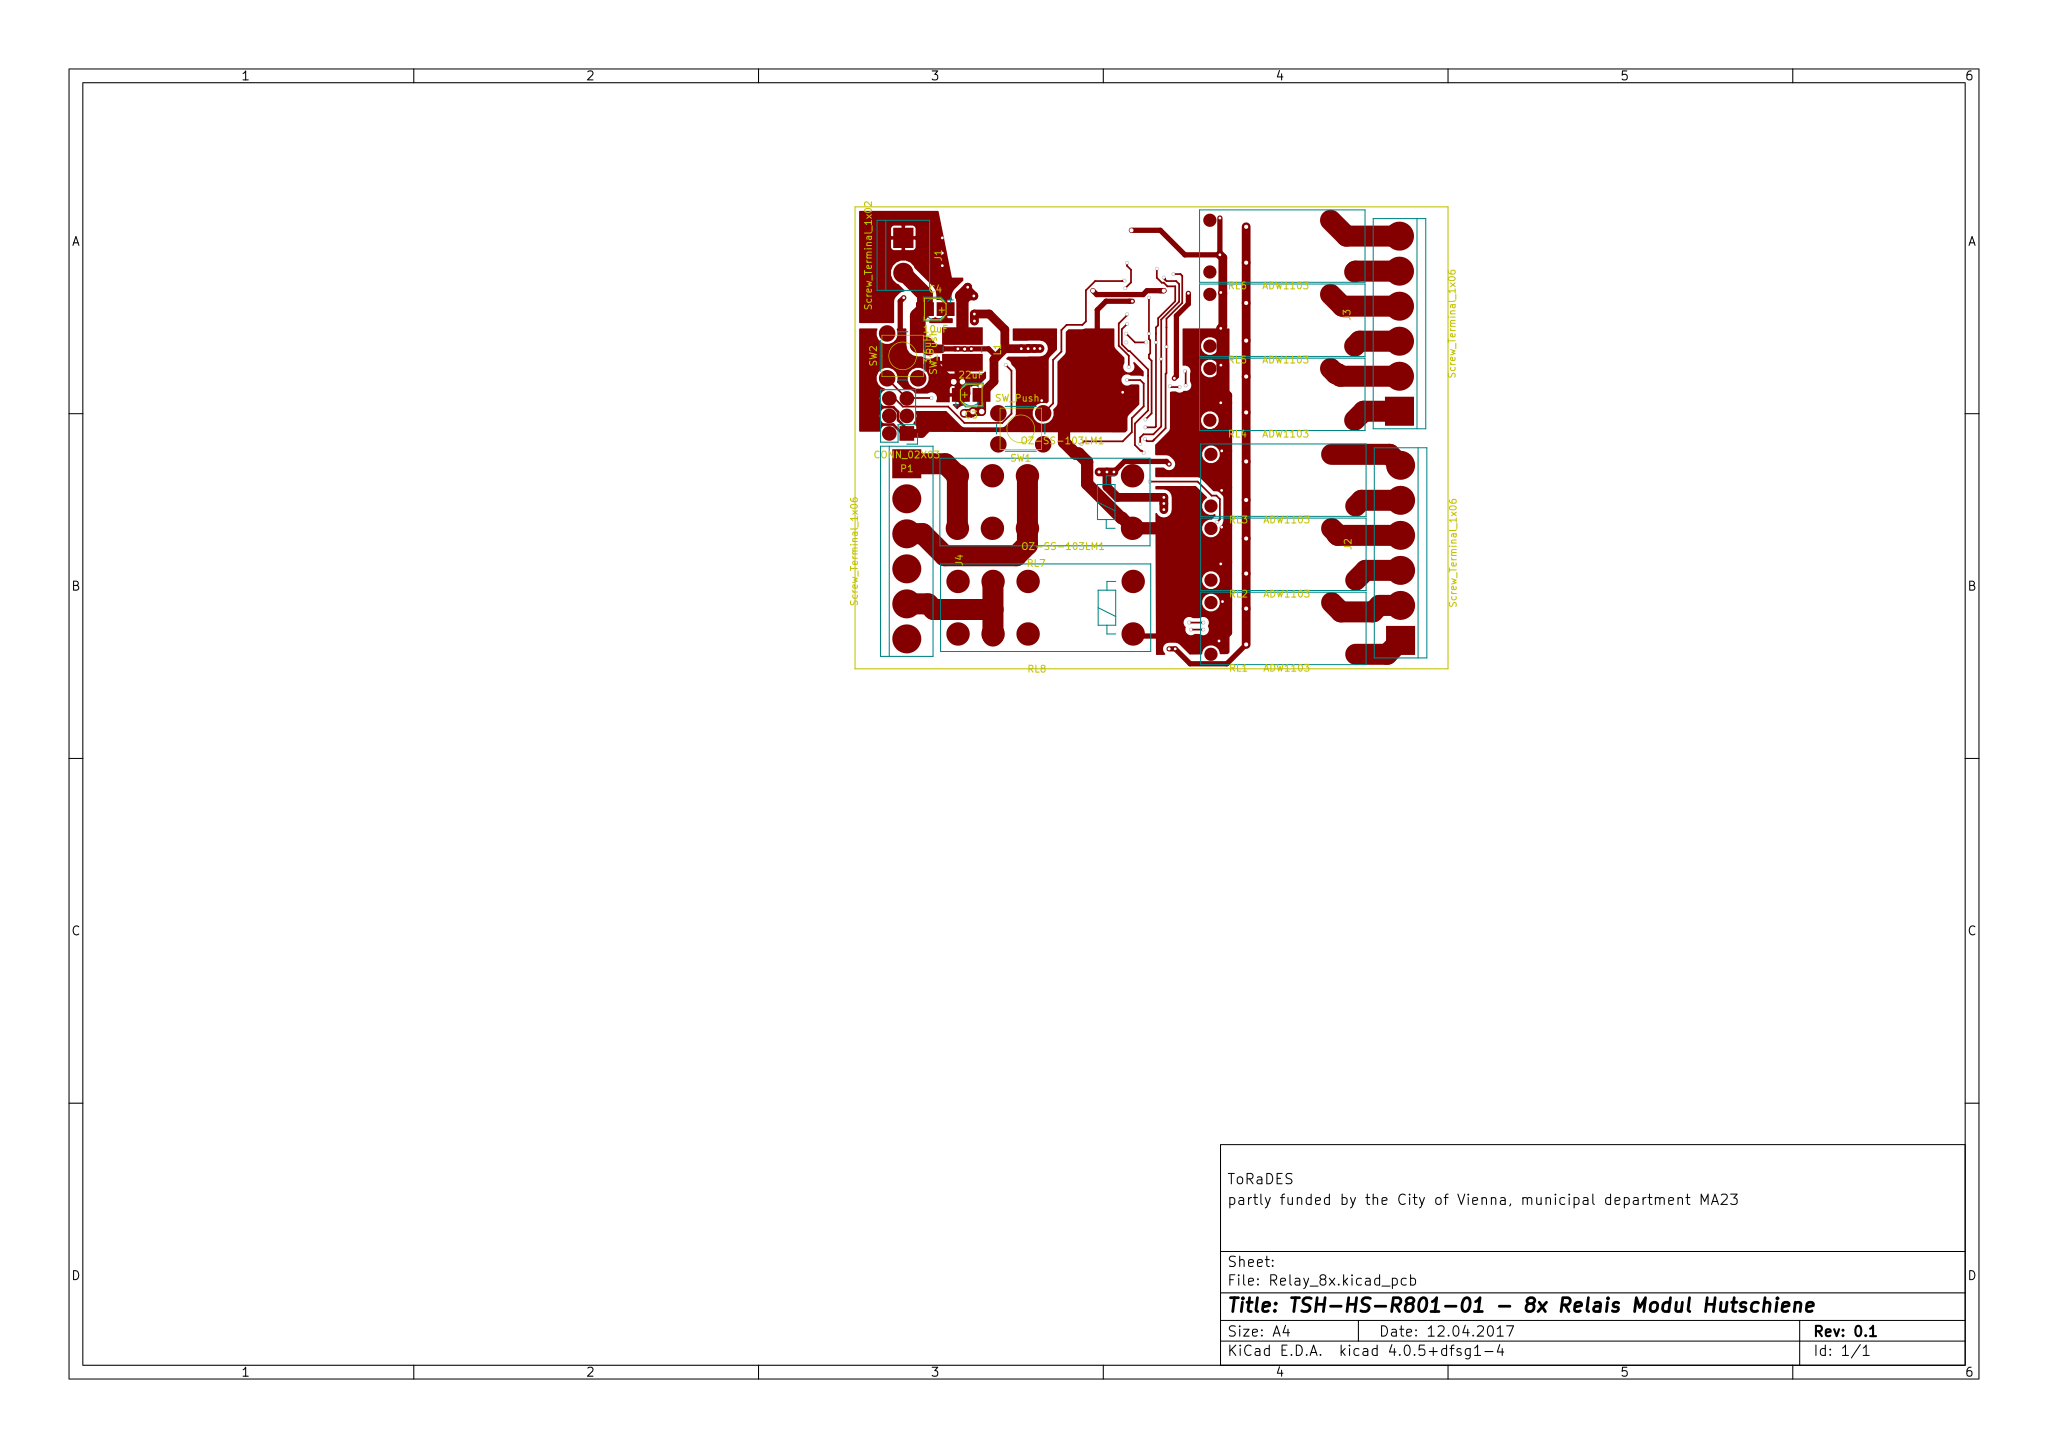
\includegraphics[width=0.95\textwidth]{img/mod/TSH-HS-R801-01-pcbF.pdf}

\subsubsection{PCB - Back}

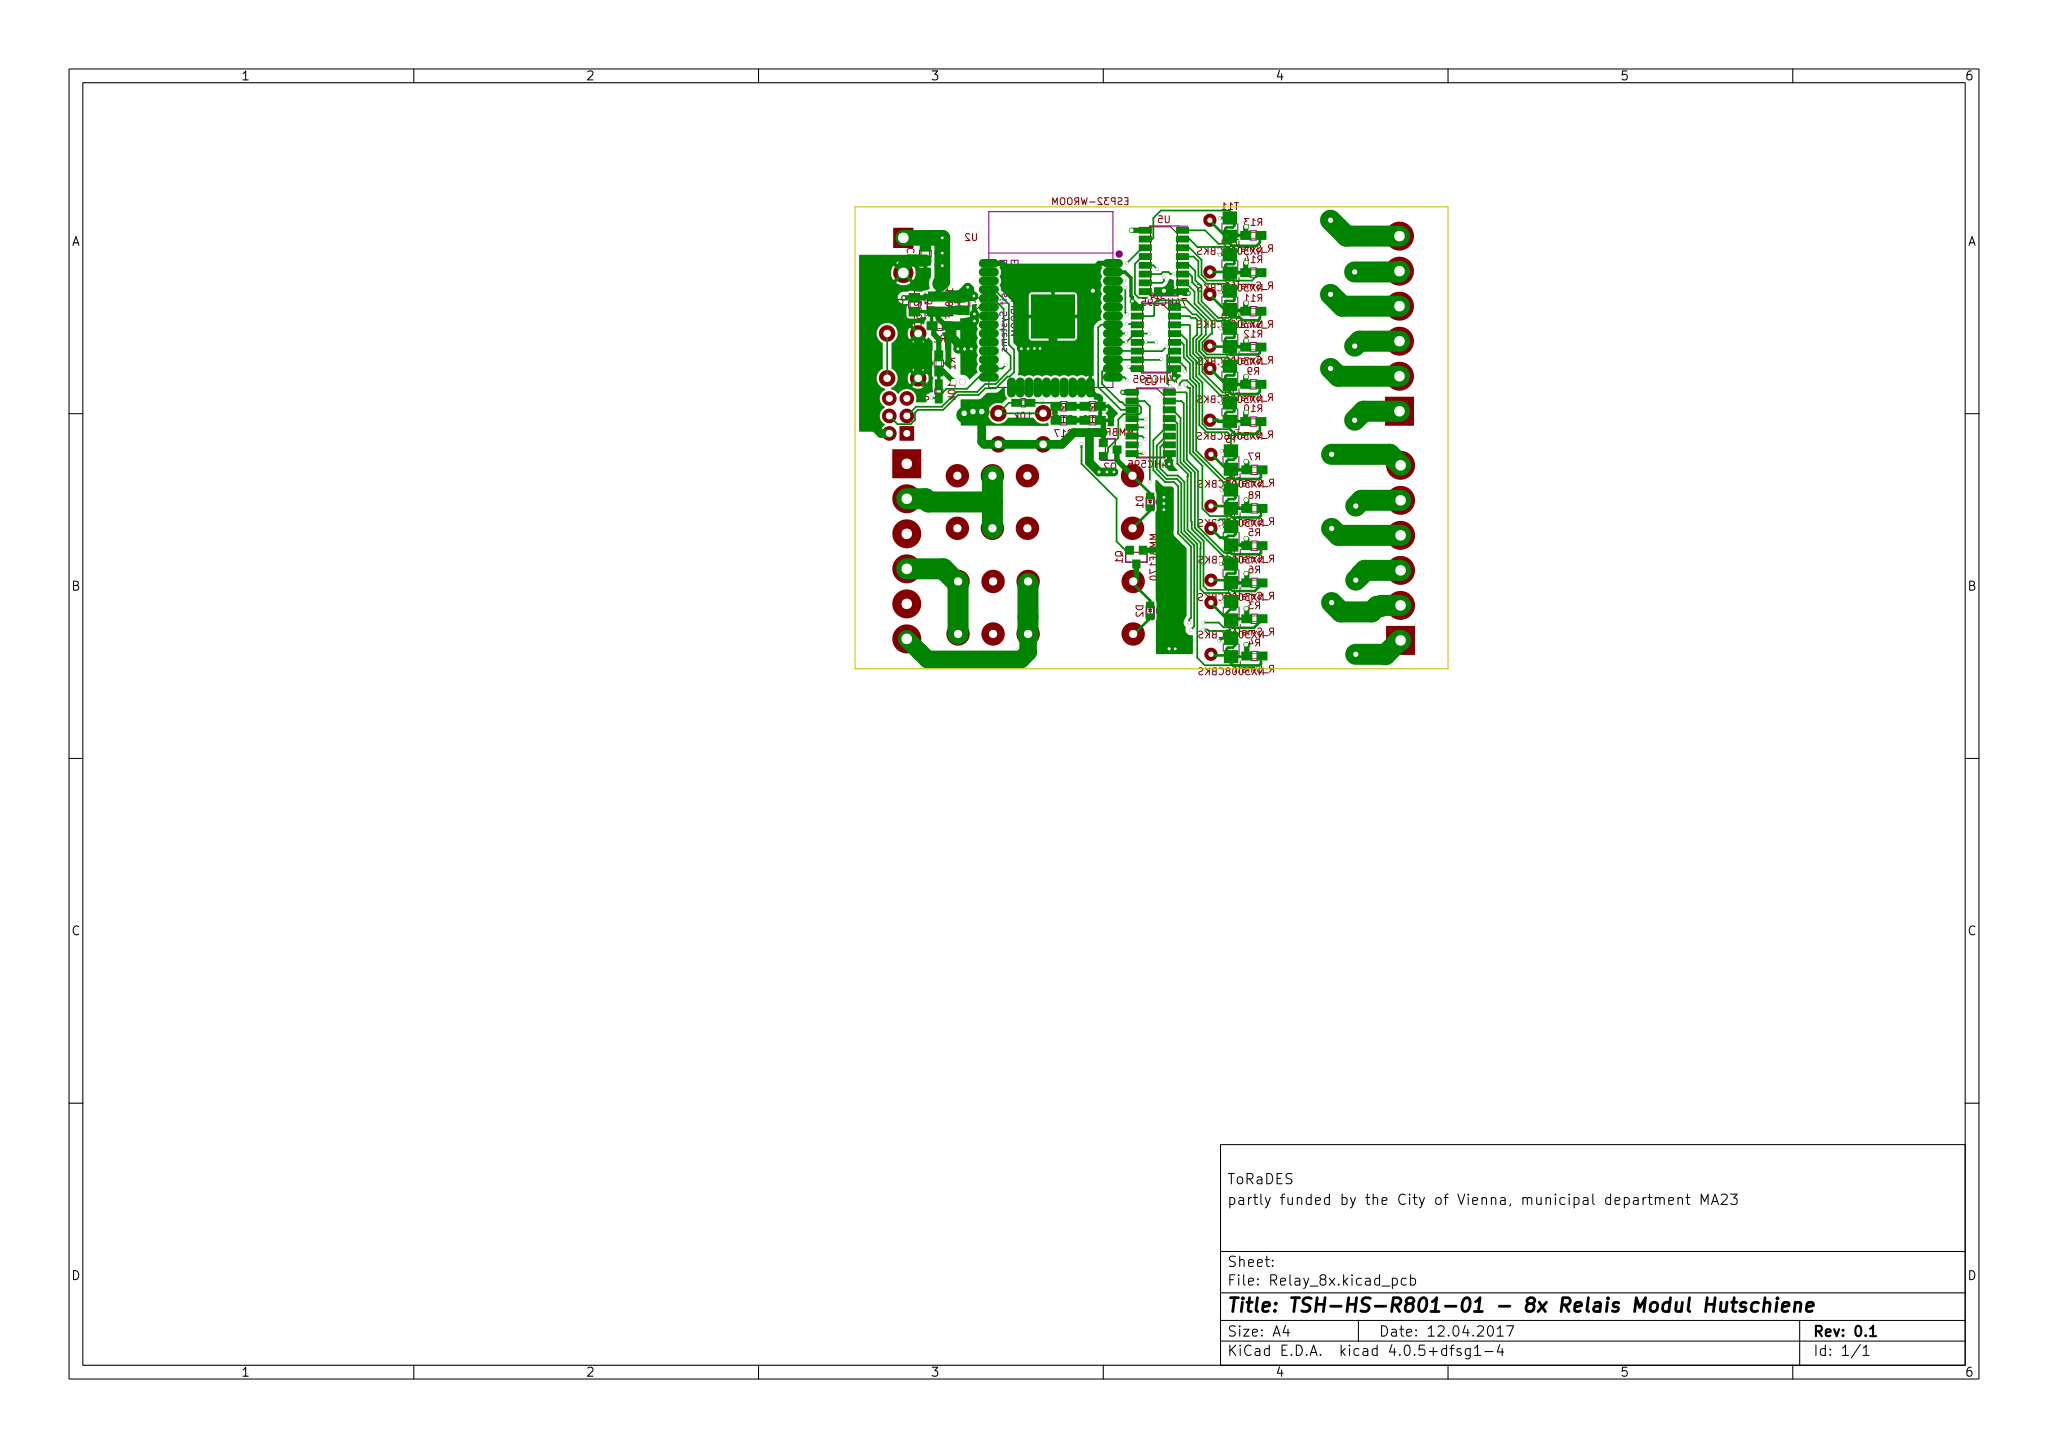
\includegraphics[width=0.95\textwidth]{img/mod/TSH-HS-R801-01-pcbB.pdf}

%%%%%%%%%%%%%%%%%%%%% NEW MODULE %%%%%%%%%%%%%%%%%%%%%%%%%%%
\newpage
\subsection{LED strip module - TSH-EX-L001-01}

\subsubsection{Specifications}

\subsubsection{MQTT - API}

\subsubsection{Applications}

\subsubsection{Schematic}

\subsubsection{PCB}

%%%%%%%%%%%%%%%%%%%%% NEW MODULE %%%%%%%%%%%%%%%%%%%%%%%%%%%

\section{Sensors}

%%%%%%%%%%%%%%%%%%%%% NEW MODULE %%%%%%%%%%%%%%%%%%%%%%%%%%%
\newpage
\subsection{Solar Powered Wall Switch - TSH-AP-SW01-01}

\begin{figure}[htb]
  \centering
  \label{img:TSH-AP-SW01-01}
  \includegraphics[width=50mm]{img/mod/TSH-AP-SW01-01.png}
  \caption{TSH-AP-SW01-01}
\end{figure}
% 
% The TSH-HS-R801-01 module is a top-hat rail (TS35) module, which provides 8 independent output. Six outputs provide a SPST-NO (single contact, normally opened) configuration,
% two outputs provide a SPDT configuration (single pole, double throw). The module is compatible with all TSH modules and uses an external power supply of 5-15VDC (max 1.5W).

The TSH-AP-SW01-01 wall mounted switch features solar powered input to any TSH solution. This version contains one rocker with individual assignment to the upper and lower action (button press).
Depending on the mounted rocker top, either one or two actuator rockers might be possible. With on rocker, there is an upper and a lower action. Two rockers enable four different input actions.
This device is fully solar powered, but it has an additional backup battery, which is used in worst case scenarios (no light for a long time). No battery consumption if there no button press.

\newpage
\subsubsection{Specifications}

The TSH-AP-SW01-01 solar powered switch provides following specifications:

\begin{table}[h!]
\centering
\label{TSH-AP-SW01-01-specs}
\begin{tabular}{|l|l|l|}
 \hline
Characteristics                                                                                  & Item                       & Specifications                                                                                                                                                                              \\ \hline \hline
\multirow{3}{*}{Dimensions}                                                                      & Width                      & 76mm	                                                                                                                                                                                    \\ 
                                                                                                 & Length                     & 76mm                                                                                                                                                                                        \\ 
                                                                                                 & Height                     & 9mm                                                                                                                                                                                         \\ \hline
\multirow{2}{*}{Mounting}                                                                        & Tape                       & 2-side adhesive tape	                                                                                                                                                                                    \\
                                                                                                 & Screws                     & 2 screws, use with 60mm wall outlets                                                                                                                                                                                        \\ \hline
\multirow{2}{*}{\begin{tabular}[c]{@{}l@{}}Electrical\end{tabular}}                              & Power                      & \begin{tabular}[c]{@{}l@{}}2x solar cells, 0.48W\end{tabular}                                                                                          \\
                                                                                                 & Current                    & 50mA during transmission \\ \hline
\end{tabular}
\end{table}

\subsubsection{MQTT - API}

TBD...
\newpage

\subsubsection{Applications}

The switch might be used in combination with different actuator modules, for example TSH-HS-R801-01.
Following use cases might be possible:
 
 \begin{itemize}
  \item Lamp switching
  \item Blindings
  \item HVAC applications
  \item ...
 \end{itemize}

\begin{center}
\includegraphics[width=80mm]{img/mod/TSH-AP-SW01-01.pdf} 
\end{center}




\subsubsection{Schematic}
  
\includegraphics[width=0.96\textwidth]{img/mod/TSH-AP-SW01-01-sch.pdf}

\begin{table}[h!]
\centering
\label{TSH-AP-SW01-01-pins}
\begin{tabular}{|l|l|l|}
\hline
WROOM pin	& Module part 	& Description \\ \hline \hline
IO25 / 10	& SW 1		& Input button 1, upper left \\ \hline
IO26 / 11	& SW 2		& Input button 2, lower left \\ \hline
IO27 / 12	& SW 3		& Input button 3, upper right \\ \hline
IO14 / 13 	& SW 4		& Input button 4, lower right \\ \hline
%TODO: Test pins description
IO4 / 26 	& GPIO$\_$SWOFF	& Switch power off \\ \hline
\end{tabular}
\caption{TSH-AP-SW01-01 ESP32 pin assignment}
\end{table}
 
\hfill \\

The solar switch is usally not powered, except the BQ25505 powered energy-harvesting circuit. Without any user-triggered action,
the energy harvester loads the SuperCap storage capacitor. When a button is pressed, the ESP32 is powered up. It is necessary to immediately read the GPIO inputs to save the 
status during the power-up.
After the power up, the necessary communication is handled and afterwards the ESP32 cuts its power supply off by pulling down the \textit{GPIO$\_$OFF} output. During operation,
this pin should be set as input. Immediately before triggering the power-cut, the input buttons should be flushed via pulling down each input button pin (to be verified!!!).


\subsubsection{PCB - Front}

\includegraphics[width=0.95\textwidth]{img/mod/TSH-AP-SW01-01-pcbF.pdf}

\subsubsection{PCB - Back}

\includegraphics[width=0.95\textwidth]{img/mod/TSH-AP-SW01-01-pcbB.pdf}

\section{Multifunctional}

\bibliographystyle{abbrv}
\bibliography{GettingStarted}

\end{document}
